\clearpage
\section{Marco conceptual}
%Con el fin de diseñar una solución para resolver la problemática redactada en el capítulo anterior, se hizo una investigación sobre el impacto que tienen las bolsas de trabajo y las bolsas de trabajo universitarias en el país. 

La Asociación de Internet MX (AIMX) es una asociación civil mexicana que tiene a los principales actores de la industria  de internet como socios y aliados. Provee información sobre distintas temáticas alrededor del mundo digital y se ha ubicado  en un marco de referencia en temas claves para el desarrollo e implementación de proyectos normativos y de política pública  que coadyuven en la productividad y la competitividad de México.\cite{amiz1}
En su último  estudio titulado ``Estudio de Búsqueda de Empleo por Internet en México 2021'', expuso que más de la mitad de los candidatos buscan trabajo en bolsas de trabajo en línea o redes sociales, ya que en los últimos dos años la pandemia a causa del virus SARS-COV2 beneficio la búsqueda digital de trabajo.\cite{AIMX}\\
    \newline

   
Más del 60\% de los mexicanos busca trabajo por internet. De una muestra de 10,864 personas tomada en el 2021, el 60\% están en el rango de edad de 25 a 39 años y predominan las personas con estudios nivel Licenciatura, es decir, la mayoría son egresados o están a punto de egresar y buscan su primer  trabajo.(Ver figura \ref{mark:pob}) 
La comunidad de ESCOM así como la comunidad politécnica entra en este rango de edad.  
\begin{figure}[H]
        \begin{center}
            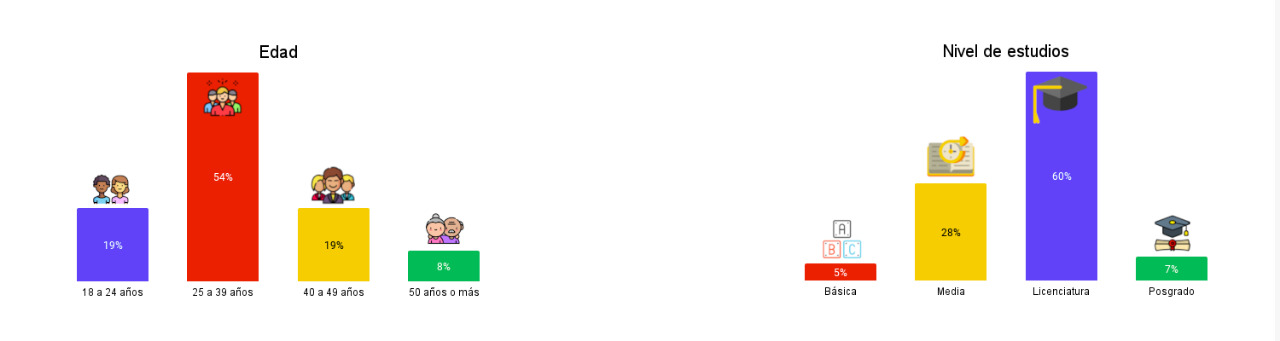
\includegraphics[width=.9\textwidth]{antecedentes/imagenes/porcen.jpeg}
        \end{center}
        \caption{Población que busca trabajo en línea.}
        \label{mark:pob}
    \end{figure}
    
El 66\% de las personas que buscan empleo o buscan una mejor oportunidad laboral tiene instalada un app de bolsa de trabajo y el 55\%  revisa vacantes en sus redes sociales, a pesar de esto, aún se mantiene a la cabeza el uso de una bolsa de trabajo en internet con el 70\% de preferencia por lo usuarios, el 87\% de las empresas buscan talento a través de estas plataformas y seis de cada 10 candidatos obtienen entrevistas gracias a ellas. \cite{AIMX}(Ver figura \ref{mark:med})

    \begin{figure}[H]
        \begin{center}
            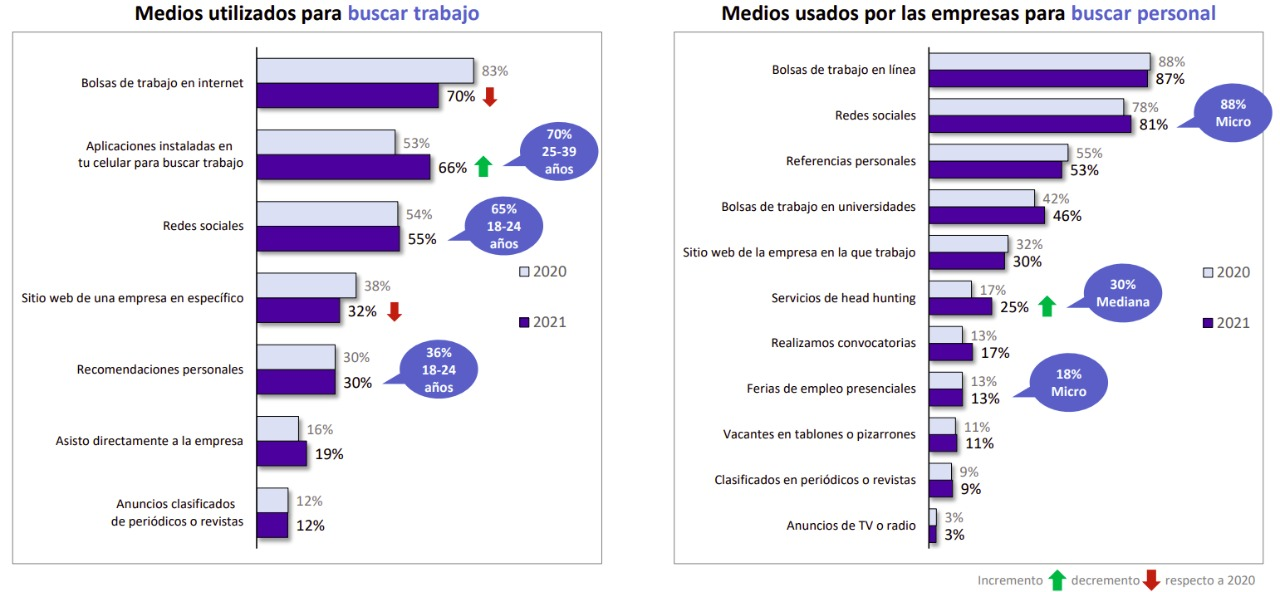
\includegraphics[width=.8\textwidth]{antecedentes/imagenes/medios.jpeg}
        \end{center}
        \caption{Medios para buscar trabajo y buscar personal AIMX 2021.}
        \label{mark:med}
    \end{figure}

 Gracias al uso de estas plataformas ha mejorado el tiempo en que un reclutador tarda en contactar a los candidatos, el principal medio es por llamada y continúa creciendo el uso de WhatsApp. Los beneficios económicos son más relevantes al evaluar una oferta de trabajo, en tanto que los reclutadores se basan más en la experiencia laboral y conocimientos. (Ver figura \ref{mark:fac})
 \\

    \begin{figure}[H]
        \begin{center}
            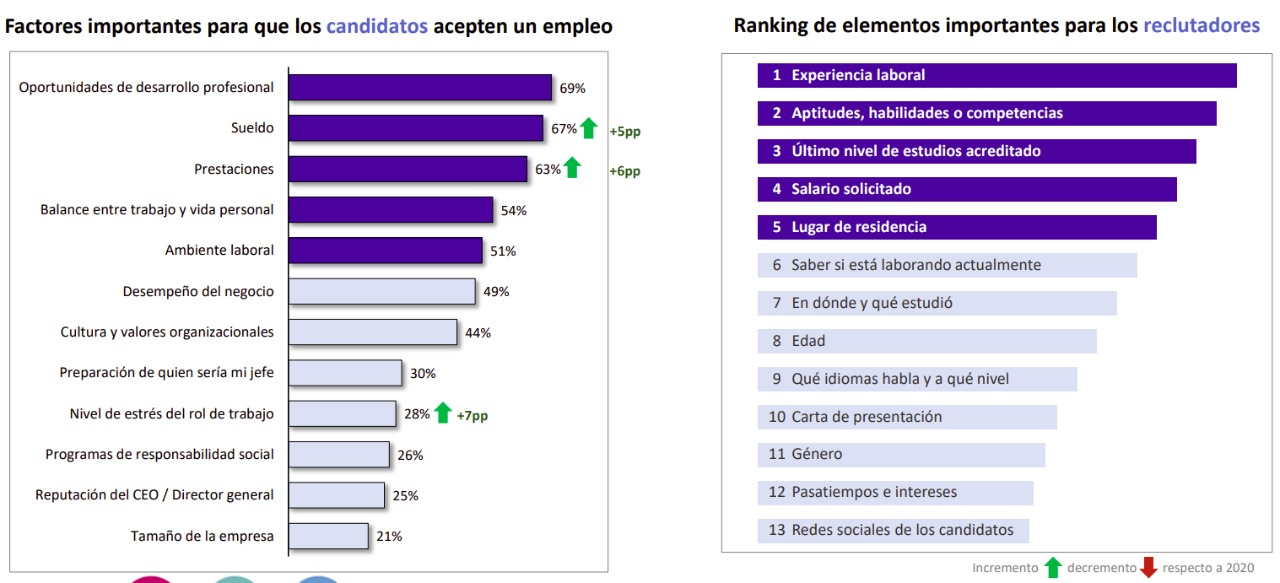
\includegraphics[width=.8\textwidth]{antecedentes/imagenes/consideraciones.jpeg}
        \end{center}
        \caption{Factores para buscar empleo y contratar personal AIMX 2021.}
        \label{mark:fac}
    \end{figure}

Por otro lado, el seguimiento de una postulación y la facilidad de postularse son los principales aspectos que buscan los candidatos en las bolsas de trabajo, aunque toma relevancia que éstas cuenten con una app. Para los reclutadores de las empresas no es tan necesario tener una aplicación móvil, ellos buscan mayormente que las bolsas de trabajo sean efectivas en la consulta de perfiles de candidatos, aunque se vuelven relevantes los aspectos relacionados a usabilidad y funciones. \cite{AIMX}\cite{Evo} (Ver figura \ref{mark:efi})
    \begin{figure}[H]
        \begin{center}
            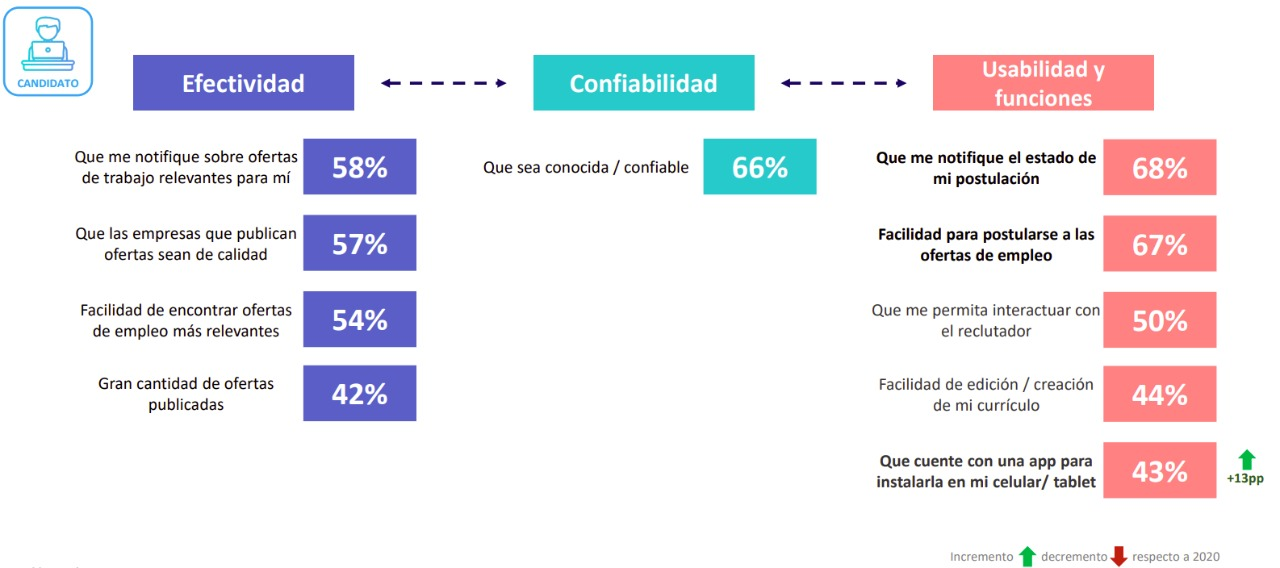
\includegraphics[width=.7\textwidth]{antecedentes/imagenes/prefC.jpeg}
            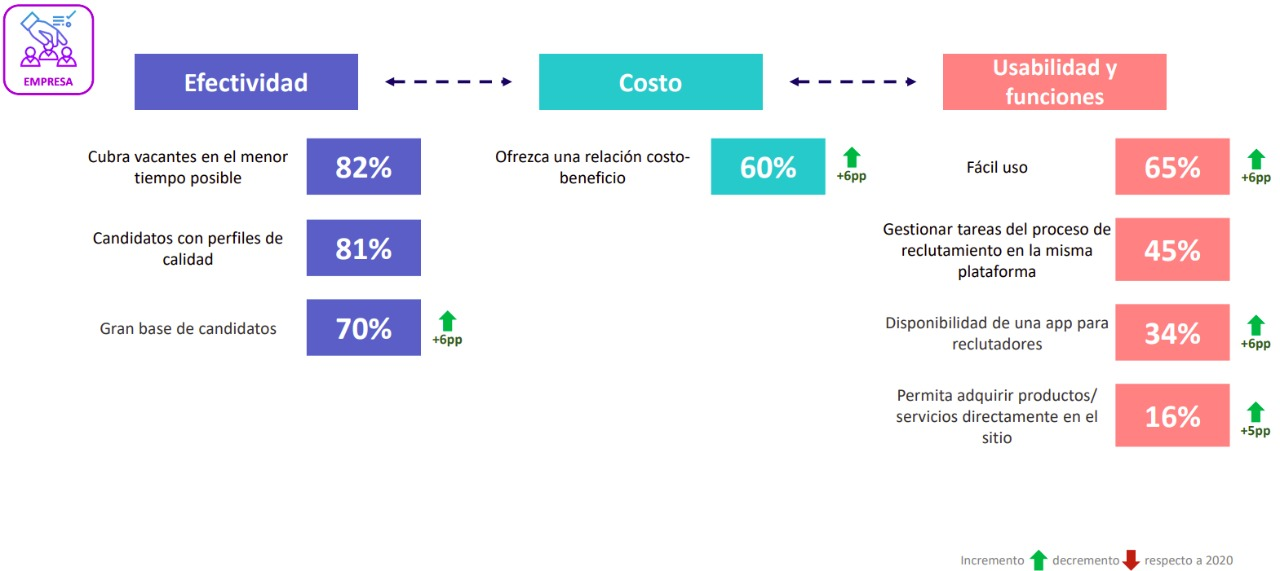
\includegraphics[width=.7\textwidth]{antecedentes/imagenes/prefE.jpeg}
        \end{center}
        \caption{Eficiencia de la plataforma para ambos usuarios.}
        \label{mark:efi}
    \end{figure}

La principal bolsa de trabajo de los candidatos y las empresas es OCC Mundial, mientras de los candidatos recurren también a las 
bolsas de empleo más populares como Computrabajo, Indeed y Linkedin los reclutadores además usan las redes sociales para buscar talento, la
figura \ref{mark:top} muestra la preferencia de plataformas por candidatos y reclutadores en el 2021.\cite{Evo}
\begin{figure}[H]
    \begin{center}
        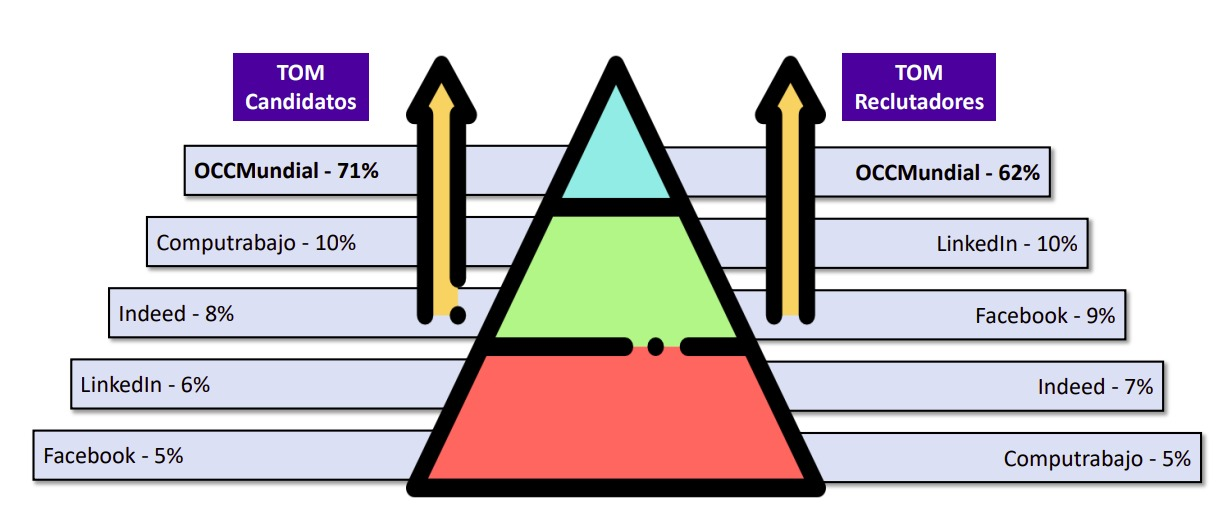
\includegraphics[width=.8\textwidth]{antecedentes/imagenes/topbdt.jpeg}
    \end{center}
    \caption{Bolsas de trabajo más populares.}
    \label{mark:top}
\end{figure}



A diferencia de las bolsas de trabajo públicas y de muchas de las privadas , las bolsas de trabajo universitarias publican empleos para sus alumnos con el fin de que puedan adquirir experiencia laboral, o bien completar créditos de libre configuración. Buscar empleo es una de las actividades que los recién egresados realizan para aplicar los conocimientos prácticos aprendidos durante su trayectoria escolar. Aunque las opciones de búsqueda son variadas siempre se enfrentan a la competencia de otros 
interesados en la misma vacante. \cite{UniJob}\\

La principal ventaja de estas bolsas de empleo universitarias es la disponibilidad de una vacante al alcance de un estudiante cuando todavía 
pertenece a la universidad. Estas ofertas, además, suelen proponer relaciones a largo plazo, y para más de una vacante. 
Como mínimo, el estudiante acumulará su primera experiencia laboral contando con el apoyo de su universidad, lo que da confianza y además, es una buena guía de inicio.
\clearpage
\subsection{Hablemos de IA y sistemas de recomendación}
    La IA es una rama de las ciencias computacionales encargada de estudiar modelos de cómputo capaces de realizar actividades propias de los seres humanos con base a dos de sus características primordiales: el razonamiento y la conducta. 1: Sin embargo, a diferencia de las personas, los dispositivos basados en IA no necesitan descansar y pueden analizar grandes volúmenes de información a la vez. Asimismo, la proporción de errores es significativamente menor en las máquinas que realizan las mismas tareas que sus contrapartes humanas.\\
    \newline
    La idea de que los ordenadores o los programas informáticos puedan tanto aprender como tomar decisiones es particularmente importante y algo sobre lo que deberíamos ser conscientes, ya que sus procesos están creciendo exponencialmente con el tiempo. Debido a estas dos capacidades, los sistemas de inteligencia artificial pueden realizar ahora muchas de las tareas que antes estaban reservadas sólo a los humanos. \\
    \newline
    Las tecnologías basadas en la IA ya están siendo utilizadas para ayudar a los humanos a beneficiarse de mejoras significativas y disfrutar de una mayor eficiencia en casi todos los ámbitos de la vida. Pero el gran crecimiento de la IA también nos obliga a estar atentos para prevenir y analizar las posibles desventajas directas o indirectas que pueda generar la proliferación de la IA. La IA se puede aplicar en casi todas las situaciones. Éstas son sólo algunas de las aplicaciones técnicas de la IA que están creciendo rápidamente en la actualidad:
    \begin{itemize}
        \item Reconocimiento de imágenes estáticas, clasificación y etiquetado:  estas herramientas son útiles para una amplia gama de industrias.
        \item Mejoras del desempeño de la estrategia algorítmica comercial: ya ha sido implementada de diversas maneras en el sector financiero.
        \item Procesamiento eficiente y escalable de datos de pacientes: esto ayudará a que la atención médica sea más efectiva y eficiente.
        \item Mantenimiento predictivo: otra herramienta ampliamente aplicable en diferentes sectores industriales.
        \item Detección y clasificación de objetos: puede verse en la industria de vehículos autónomos, aunque también tiene potencial para muchos otros campos.
        \item Distribución de contenido en las redes sociales: se trata principalmente de una herramienta de marketing utilizada en las redes sociales, pero también puede usarse para crear conciencia entre las organizaciones sin ánimo de lucro o para difundir información rápidamente como servicio público.
        \item Protección contra amenazas de seguridad cibernética: es una herramienta importante para los bancos y los sistemas que envían y reciben pagos en línea.
    \end{itemize}

    El aprendizaje automático (en inglés, machine learning) es uno de los enfoques principales de la inteligencia artificial. En pocas palabras, se trata de un aspecto de la informática en el que los ordenadores o las máquinas tienen la capacidad de aprender sin estar programados para ello. Un resultado típico serían las sugerencias o predicciones en una situación particular. Gracias al aprendizaje automático, muchos de los dispositivos que verás en el futuro obtendrán experiencia y conocimientos a partir de la forma en que son utilizados para poder ofrecer una experiencia al usuario personalizada.\\
    \newline
    El aprendizaje automático usa algoritmos para aprender patrones de datos. Por ejemplo, los filtros de spam de correo electrónico utilizan este tipo de aprendizaje con el fin de detectar qué mensajes son correo basura y separarlos de aquellos que no lo son. Éste es un sencillo ejemplo de cómo los algoritmos pueden usarse para aprender patrones y utilizar el conocimiento adquirido para tomar decisiones.\\
    \newline
    Existen tres subconjuntos del aprendizaje automático que pueden utilizarse: aprendizaje supervisado, no supervisado y de refuerzo:
    \begin{itemize}
        \item  \textit{Aprendizaje supervisado:} los algoritmos usan datos que ya han sido etiquetados u organizados previamente para indicar cómo tendría que ser categorizada la nueva información. Con este método, se requiere la intervención humana para proporcionar retroalimentación.
        \item  \textit{Aprendizaje no supervisado:} los algoritmos no usan ningún dato etiquetado u organizado previamente para indicar cómo tendría que ser categorizada la nueva información, sino que tienen que encontrar la manera de clasificarlas ellos mismos. Por tanto, este método no requiere la intervención humana
        \item  \textit{Aprendizaje por refuerzo:}los algoritmos aprenden de la experiencia. En otras palabras, tenemos que darles «un refuerzo positivo» cada vez que aciertan. La forma en que estos algoritmos aprenden se puede comparar con la de los perros cuando les damos «recompensas» al aprender a sentarse.
    \end{itemize}
    
    Los sistemas de recomendación están en todas partes. Impulsan muchos de los servicios que nos encantan y que usamos todos los días. 
    Desde hacer compras hasta el streaming y el uso de los motores de búsqueda, los sistemas de recomendación están diseñados para 
    ayudar a las personas a tener una experiencia más personalizada.\\
    \newline
    Un sistema de recomendación es aquél que produce una lista de sugerencias para un usuario. Cada objeto de la lista se llama “ítem” 
    de manera genérica, pues dichas sugerencias pueden ser artículos, películas, música, etc.\\
    \newline
    Aunque todos los sistemas de recomendación tienen el mismo objetivo final, difieren en aspectos como la información utilizada para 
    hacer recomendaciones y en el funcionamiento del algoritmo. A continuación, se presentan las clasificaciones más comunes.
    
    \begin{description}
        \item[Filtrado colaborativo] En esta categoría se intenta predecir la “clasificación” de un ítem para un usuario con base en las 
        clasificaciones de otros usuarios; se encuentran personas con gustos (clasificaciones) similares al usuario y se le recomiendan 
        ítems que les gusten a esas personas.\\
        \newline

    Uno de los problemas más grandes en este tipo de recomendación es la falta de información, pues no todos los usuarios han 
    clasificado todos los ítems. En la mayoría de los casos, los usuarios acceden (y clasifican) los ítems que les gustan. Otro problema
    es el cold start (inicio frío); es difícil recomendar ítems nuevos debido a falta de clasificaciones y también es difícil hacer 
     recomendaciones a un usuario nuevo por la falta de historial de clasificaciones. \cite{mc1}
        \item[Basado en contenido] Los sistemas de recomendación basados en contenido hacen sus recomendaciones con base en descripciones de los 
    ítems y los intereses del usuario. Cada ítem tiene atributos, y se determina su similitud con otros ítems dependiendo de los 
    atributos que compartan. Por ejemplo, si a un usuario le gustan películas del género “Acción”, el sistema recomendaría más películas de ese mismo género.\\
    \newline
    Un problema con los sistemas basados en contenido es que los ítems no tengan suficientes atributos para ser diferenciados por el 
    sistema de acuerdo con un usuario. Por ejemplo, aunque al usuario le gusten las películas de acción, no quiere decir que le gusten 
    todas las películas de este género; quizá no le gustan las películas con finales tristes, pero el sistema no tenía ese atributo 
    contemplado. \cite{mc4}
    
    \item[Demográficos] Este tipo de sistema toma en cuenta datos del perfil demográfico de un usuario. Por ejemplo, se pueden hacer recomendaciones basadas en la región o país del usuario, o recomendar con base en la edad del usuario.\cite{mc5}
    \item[Híbridos] Como el nombre indica, son aquellos que combinan aspectos de diferentes tipos de sistemas de recomendación. Hoy en día son el tipo más común, pues se intenta minimizar las desventajas de algún tipo con la inclusión de aspectos de otro tipo.
    
    
    \end{description}
    \textbf{Beneficios de implementar sistemas de recomendación en bolsas de trabajo}\\
    Los sistemas de recomendación han logrado cambiar la forma en la que consumimos nuevos contenidos y descubrimos productos nuevos. Uno de los ejemplos más claros los podemos disfrutar en las páginas de compra de productos como Amazon o Mercado Libre. Con un nivel de precisión alto, estos sistemas web con algunos pocos datos pueden proporcionarnos de sugerencias de productos adaptadas a nuestras necesidades. De igual forma sucede con las plataformas de contenidos como YouTube, Spotify o Netflix. Sus recomendaciones precisas nos ayudan a descubrir nuevas series, videos o artistas al analizar nuestros gustos y preferencias.\\
    \newline
    Esto se traduce en una mejor satisfacción de las necesidades del cliente. La experiencia del usuario se convierte en una actividad más agradable, ya que estos sistemas actúan como un asistente personal que estimula a la persona a seguir descubriendo elementos. Adicionalmente estos sistemas aportan una eficiencia excepcional a las conversiones de los sitios web. Las recomendaciones de productos personalizados acerca al cliente a lo que desea, mejorando las posibilidades de que este efectivamente compre o consuma el contenido sugerido. \cite{mc6}
    
    %Desde ya hace tiempo, las empresas y bolsas de trabajo utilizan escáneres de currículums o como otros le llaman ATS  (Applicant Traking System ) su objetivo es acelerar su proceso de contratación y filtrar automáticamente los currículums que no parecen ser adecuados para el trabajo, de acuerdo al articulo de Linkedin 
    %más del noventa por ciento de los currículums se descartan antes de que lleguen a un gerente de contratación o un reclutador, sin ni siquiera ser mirados por una persona.
    
   % El proceso automatizado de selección de currículums puede ser injusto para los solicitantes de empleo y más para aquellos que apenas van empezando. Después de todo, las personas que buscan empleo, han pasado un buen rato haciendo el currículum perfecto, sin embargo, una bolsa de empleo permite que un algoritmo decida si puede ser entrevistarlo o no.
 
    %La razón es que una publicación de una vacante promedio recibe demasiadas solicitudes no calificadas (más del 80\%). Por ejemplo, un empleador que contrata para un puesto de finanzas puede obtener solicitantes que no tengan experiencia en el área financiera o de otras áreas. Este suele ser el resultado de personas que se postulan en masa para todos los trabajos que ven con el mismo currículum o aquellos que creen en el "chicle y pega". Las ATS les ayuda a filtrar a muchos de estos solicitantes no calificados.
    